\section{Installazione e avvio}
\subsection{Requisiti Server}
\noindent Per utilizzare il server è necessario:
\begin{itemize}[label=-]
  \item Installare \href{https://dev.mysql.com/downloads/installer/}{MySQL} sul proprio computer
  \item Eseguire lo script sql presente nel percorso "\textbackslash KmeansServer\textbackslash out\textbackslash artifacts\textbackslash KmeansServer\_jar"
  \\ \textbf{Esempio}: \textbackslash . C:\textbackslash Users\textbackslash acurr\textbackslash Desktop\textbackslash KmeansBase\textbackslash KmeansServer\textbackslash out\textbackslash artifacts\textbackslash KmeansServer\_jar\textbackslash script.sql
  \\ Digitando questo comando sulla shell di MySQL sarà creato il database e le tabelle necessarie.
  \item Installare \href{https://www.oracle.com/technetwork/java/javase/downloads/jre8-downloads-2133155.html}{JRE} 8
  \item Installare JDK 19.0.2(?)
\end{itemize}

\subsection{Requisiti Client}
\subsubsection{CLI}
\noindent Per utilizzare il client è necessario:
\begin{itemize}[label=-]
  \item Installare \href{https://www.oracle.com/technetwork/java/javase/downloads/jre8-downloads-2133155.html}{JRE} 8  
  \item Server in ascolto
\end{itemize}

\subsubsection{App}
\noindent Per utilizzare il client app è necessario:
\begin{itemize}[label=-]
  \item Un dispositivo Android con sistema operativo Android 5.0 Lollipop o superiore
  \item Installare l'applicazione: trasferire l'APK sullo smartphone (\textbf{percorso APK}). Aprire il file APK e installare l'applicazione. Se necessario abilitare l'installazione di applicazioni da sorgenti sconosciute e dare l'ok nel caso in cui l'installazione venga bloccata da Play Protect.
  \item Server in ascolto
\end{itemize}


\subsection{Avvio server}
\subsubsection{CLI}
\noindent Per avviare il server e' necessario eseguire il file \textit{server.bat} nella stessa cartella di \textit{server.jar}. In alternativa è possibile avviarlo da riga di comando tramite il comando \textit{java -jar server.jar}.

\subsubsection{App}
\noindent

\subsection{Avvio client}
\subsubsection{CLI}
\noindent Per avviare il client da riga di comando è necessario eseguire il file \textit{client.bat} nella stessa cartella del file \textit{client.jar}. Questa modalità di avvio connetterà il client ad un server in esecuzione sulla propria macchina sulla porta 8080. Per specificare un altro server a cui connettersi è necessario
avviare il client da riga di comando tramite il comando \textit{java -jar client.jar indirizzo\_ip porta} o inserendo tale comando nel file batch.


\subsubsection{App}
\noindent Per avviare il client app basta avviare l'applicazione sul proprio smartphone ed inserire indirizzo ip e porta del server a cui ci si vuole connettere:
\begin{figure}[H]
  \centering
  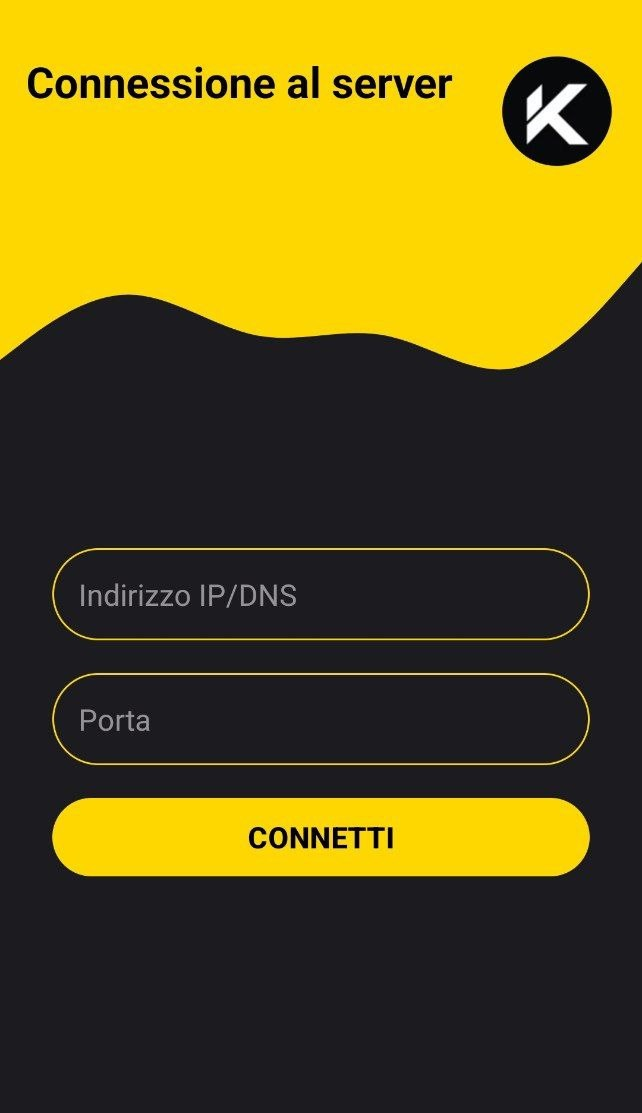
\includegraphics[scale=0.25]{img/app1.png}
  \caption{Schermata iniziale dell'applicazione}
\end{figure}
